\section{Quick prototype}

We implemented our fast technique for Pointproofs using \textsf{libff}~\cite{libff}.
We also implemented the Feist and Khovratovich (FK)~\cite{FK20} technique for computing all proofs in KZG-based VCs~\cite{TAB+20}.
Our code is available at:
\begin{center}
    \url{https://github.com/alinush/libvectcom}
\end{center}

\noindent We ran three benchmarks on a Macbook Pro with a 2.4 GHz 8-Core Intel Core i9 and 32 GB of RAM, for different vectors of size $N=2,4,8,16,\dots,1024$.
We measured:
\begin{itemize}
    \item Our fast $O(N\log{N})$-time proof precomputation in Pointproofs from \cref{s:pointproofs:precompute-all-proofs},
    \item The naive $O(N^2)$-time proof precomputation for Pointproofs,
    \item The fast $O(N\log{N})$-time proof precomputation for KZG-based VCs via the FK technique.
\end{itemize}

\noindent We plot the results in \cref{f:benchmarks}.
We find that our $O(N\log{N})$ algorithm for Pointproofs scales much better than the naive, $O(N^2)$ one.
We also find that computing all proofs in Pointproofs using our algorithm is slightly faster than computing all proofs in KZG-based VCs using the FK technique.
This is because the FK techniques requires an additional DFT on group elements.

\begin{figure}[t]
    \centering
    \textbf{Precomputing all $N$ proofs in Pointproofs and in KZG-based VCs}
    \par
    \medskip
    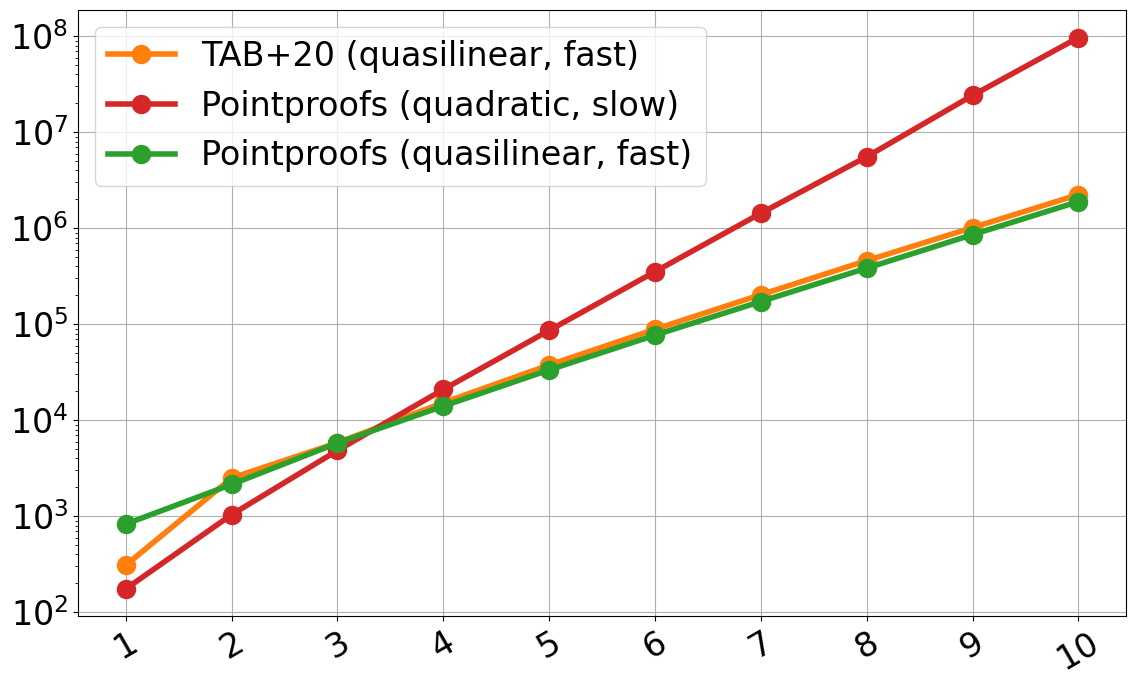
\includegraphics[width=0.50\columnwidth]{fk-vs-pointproofs.png}
    \caption{
        The $x$-axis is $\log_2{N}$, where $N$ is the size of the vector of messages $\vect{m}$.
        The $y$-axis is the time to compute all $N$ proofs for the specified scheme, in microseconds.
    }
    \label{f:benchmarks}
\end{figure}
